%%%%%%%%%%%%%%%%%%%%%%%%%%%%%%%%%%%%%%%%%%%%%%%%%
%%%%%%%%%%%% cap: intro %%%%%%%%%%%%%%%%%
%%%%%%%%%%%%%%%%%%%%%%%%%%%%%%%%%%%%%%%%%%%%%%%%%

\chapter{Introduction}\label{cap:intro}

%%%%%%%%%%%% Section: Description %%%%%%%%%%%%

\hspace{\parindent}Managing finances can be a challenge for many people, especially for those who have never received proper education on financial management. Poor financial management can lead to debt, and financial stress, which can negatively impact one's quality of life.

\hspace{\parindent}One of the biggest issues with money management is the lack of financial education. Many people have never been taught how to properly manage their finances, leading to poor spending habits, lack of savings, and accumulating debt. Without the proper knowledge and skills, it can be difficult to make informed financial decisions and plan for the future.

\hspace{\parindent}Another problem is that many people live beyond their means, which means they spend more money than they earn. This can lead to accumulating debt and struggling to make ends meet. Living beyond one's means can also prevent individuals from saving money for future expenses or emergencies.

\hspace{\parindent}Savings are important because they provide a safety net for unexpected expenses and can help individuals achieve their long-term financial goals. Having savings can also reduce financial stress and provide a sense of security. However, managing finances can be a challenge for various people, especially those who lack proper financial education. Poor financial management can lead to debt and financial stress, negatively impacting one’s quality of life.

\hspace{\parindent}Managing finances can be a challenge for many people, especially for those who have never received proper education on financial management. Poor financial management can lead to debt, and financial stress, which can negatively impact one's quality of life.

% \hspace{\parindent}Savings are important because they provide a safety net for unexpected expenses and can help individuals achieve their long-term financial goals. Having savings can also reduce financial stress and provide a sense of security. However, managing finances can be a challenge for various people, especially those who lack proper financial education. Poor financial management can lead to debt and financial stress, negatively impacting one’s quality of life.

\hspace{\parindent}The lack of financial education is a major issue, as many individuals have never been taught how to manage their finances effectively. Accumulating debt is a consequence of poor spending habits and a lack of savings. Spending beyond one’s means can cause financial hardship, making it difficult to save and pay bills.

\hspace{\parindent}Savings are crucial for providing a safety net for unexpected expenses and achieving long-term financial goals. They reduce financial stress and provide a sense of security. A lack of financial education, overspending, and neglecting to prioritize savings all contribute to people's difficulty in saving money.

\hspace{\parindent}While there are money management applications available, they often lack comprehensiveness and personalization. Complex applications lack user-friendliness and the ability to meet varied needs. They may be difficult to use or overwhelm users with unnecessary features. The proposed application focuses on user-friendly design, prioritizes key features, and provides relevant financial education resources User-friendliness and a visually appealing interface are crucial for the success of an application. There is a requirement for a mobile app that offers an effective and user-friendly solution for personal finance management. The application should have a personalized approach, offer relevant financial education, and promote long-term financial stability and well-being.

\hspace{\parindent}A mobile platform has been proposed to provide an easy-to-use and intuitive financial management experience. The interface prioritizes usability and simplicity, with clear navigation and visual elements. The application incorporates features to promote financial education, offering tips and resources for saving money, investing wisely, and making informed financial decisions.

\hspace{\parindent}By offering a comprehensive approach to financial management, the mobile app stands out. It's possible to add transactions, generate reports, monitor expenses, and set savings goals through this service. The application aims to help users develop better financial habits and achieve their goals.


\hspace{\parindent}The lack of financial education is a major issue, as many individuals have never been taught how to manage their finances effectively. Accumulating debt is a consequence of poor spending habits and a lack of savings. Spending beyond one’s means can cause financial hardship, making it difficult to save and pay bills.

\hspace{\parindent}Savings are crucial for providing a safety net for unexpected expenses and achieving long-term financial goals. They reduce financial stress and provide a sense of security. A lack of financial education, overspending, and neglecting to prioritize savings all contribute to people's difficulty in saving money.

\hspace{\parindent}While there are money management applications available, they often lack comprehensiveness and personalization. Complex applications lack user-friendliness and the ability to meet varied needs. User-friendliness and a visually appealing interface are crucial for the success of an application. There is a requirement for a mobile app that offers an effective and user-friendly solution for personal finance management. The application should have a personalized approach, offer relevant financial education, and promote long-term financial stability and well-being.

\hspace{\parindent}A mobile platform has been proposed to provide an easy-to-use and intuitive financial management experience. The interface prioritizes usability and simplicity, with clear navigation and visual elements. The application incorporates features to promote financial education, offering tips and resources for saving money, investing wisely, and making informed financial decisions.

\hspace{\parindent}By offering a comprehensive approach to financial management, the mobile app stands out. It's possible to add transactions, generate reports, monitor expenses, and set savings goals through this service. The application aims to help users develop better financial habits and achieve their goals.

\hspace{\parindent}The proposed application focuses on user-friendly design, prioritizes key features, and provides relevant financial education resources.

\hspace{\parindent}Two similar solutions, BlueCoins, and Money Lover are compared. BlueCoins offers customization and detailed tracking but may be overwhelming for casual users. Money Lover emphasizes user experience but hypes paid features, which may not be accessible to all users. Revolut, although not a direct competitor, is mentioned for its popularity and user-friendly interface.

% NOT SURE ABOUT THIS ONE%
% \hspace{\parindent}In conclusion, the proposed mobile application offers a unique solution for personal finance management. It provides user-friendly design and tailored features, ideal for long-term objectives.
% \vspace*{2mm}


%%%%%%%%%%%% Section: Motivation %%%%%%%%%%%%
\newpage
\section{Proposed Solution}\label{sect: Motivation}
\hspace{\parindent} The application is user-friendly and provides an intuitive experience for managing finances. Clear navigation and visual elements are used in the user interface to prioritize usability and simplicity, enhancing user experience. The application aims to provide users with the tools and resources to manage their finances efficiently and effectively.

\hspace{\parindent}Besides its user-friendly interface, the application incorporates features to promote financial education and literacy. It provides users with tips and resources for saving money, investing wisely, and making informed financial decisions. Financial literacy is essential for individuals to make smart financial decisions.

\hspace{\parindent}The proposed mobile application is unique in its comprehensive approach to managing personal finances, offering users a range of features that are tailored to their specific needs. From adding transactions and generating reports to monitor expenses and setting savings goals, the application offers a full suite of tools and resources to help users achieve their financial goals.

\hspace{\parindent}Overall, the proposed mobile application offers a powerful combination of user-friendly design and financial education resources, making it an ideal tool for individuals seeking to improve their financial management skills and achieve their long-term financial goals.

%%%%%%%%%%% Section: Similar Solutions %%%%%%%%%%%%
\section{State of the art}\label{sect:State of the art}
\hspace{\parindent} Although there are a plethora of money management applications available in the market, the proposed application stands out from the rest because of its exceptional level of customization and personalization, which many other applications cannot provide. In addition, some applications may be difficult to use or have a steep learning curve, which can deter users from using them effectively.

\hspace{\parindent}In order to address this gap, the proposed application has been developed to feature a user-friendly interface that considers the principles of both UI and UX. The application has been designed with the user in mind, and it is geared towards making sure that users can perform tasks with no difficulties. These tasks include navigation, transaction addition, report generation, and expense monitoring.

\hspace{\parindent}Moreover, the proposed application goes beyond simply tracking expenses by also providing educational resources and tips for saving money. This is important as many people struggle with managing their finances due to a lack of financial education. By incorporating educational features, the proposed application aims to help users develop better financial habits and achieve their financial goals.


\hspace{\parindent}While many comparable solutions exist, a significant number of them suffer from "feature creep", which arises when an excessive number of features are added without proper consideration given to how they will impact usability and user experience. The whole purpose of a money management tool is to make it easier for users to manage their finances, but if the application is confusing and overwhelming, it defeats this purpose altogether. The issue at hand is being tackled with our proposed mobile application that gives top priority to a user-friendly interface and concentrates on the key features that are most vital for effective financial management.


\hspace{\parindent}In contrast to other money management solutions, the proposed application takes a distinctive and comprehensive approach that prioritizes user experience and education.


\subsection{BlueCoins}
\hspace{\parindent}BlueCoins, a comprehensive money management application, offers a wide range of features that meet the power users’ needs. Although this application may be appropriate for advanced users who need a wide range of customization and intricate financial monitoring, it might not be the ideal option for every user, specifically those who prioritize the user-friendliness and simplicity of their financial management apps.

\hspace{\parindent}One of the main advantages of BlueCoins is its ability to allow users to create custom categories for expenses and set limits for each category to stay within their budget. It also offers features such as transaction categorization, budget forecasting, and reports. Users can also create recurring transactions for monthly expenses such as rent or bills

\hspace{\parindent}Despite its various features, the app's lack of focus on user experience may lead to decreased interest from casual users who are seeking a simple and efficient method for managing their finances. The application may experience a phenomenon known as "feature creep," which refers to the situation where various features are continually added to the program, resulting in increased complexity and making it overwhelming for some users.

\hspace{\parindent}Although BlueCoins is equipped with detailed financial tracking and an extensive range of customization options, users who value simplicity and a user-friendly interface may not find it to be the best fit for their financial management needs.
\begin{figure}[htbp]
  \centering
  \begin{minipage}[b]{0.24\textwidth}
    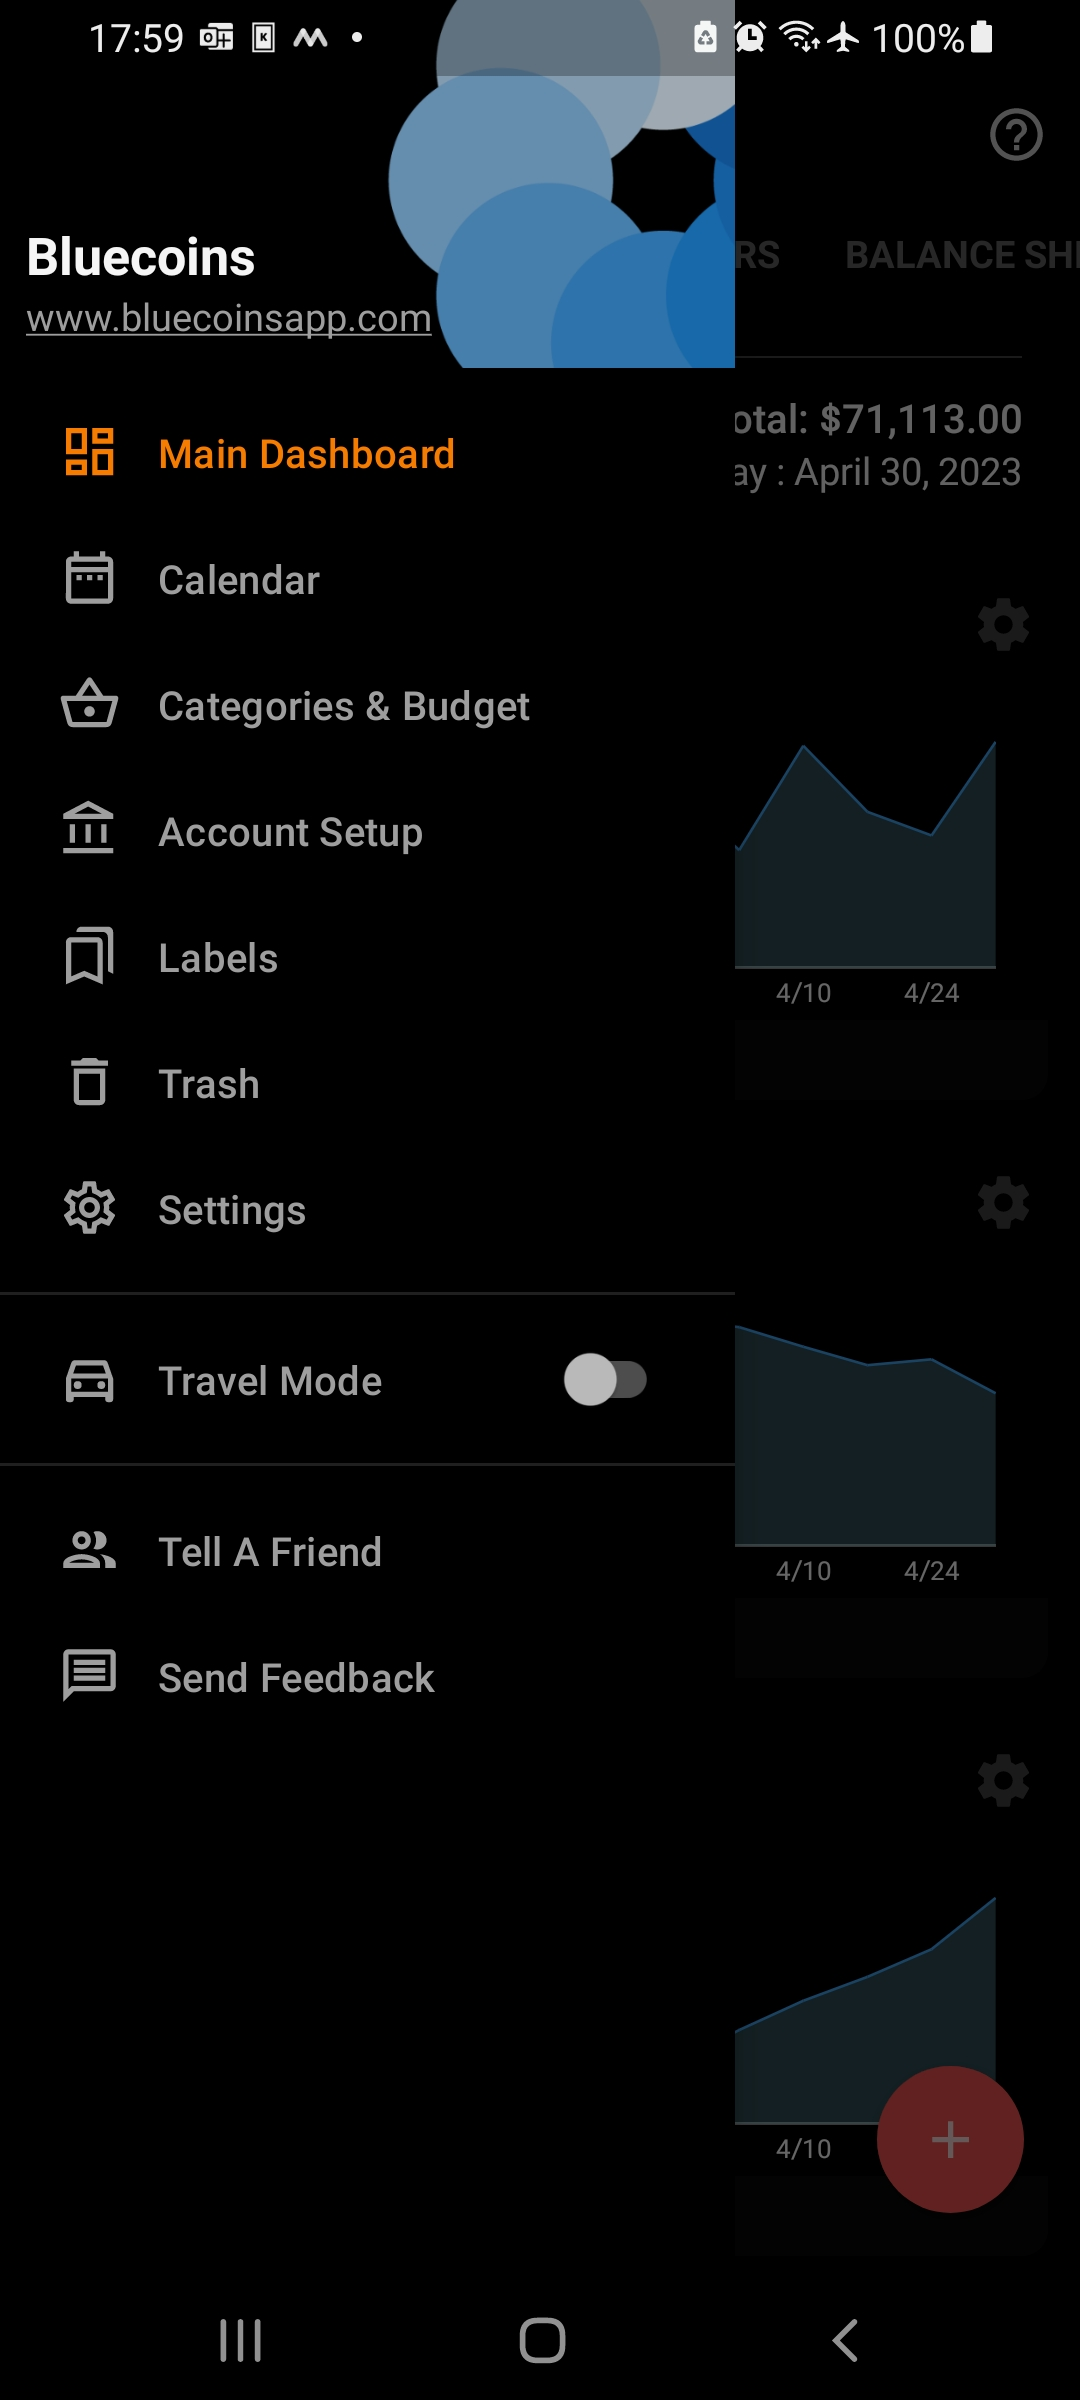
\includegraphics[width=\textwidth]{Screen Shots/BlueCoins/D_MainMenu.jpg}
    \caption{Blue Coins Dark main menu 1.}
    \label{fig:image1}
  \end{minipage}
  \hfill
  \begin{minipage}[b]{0.24\textwidth}
    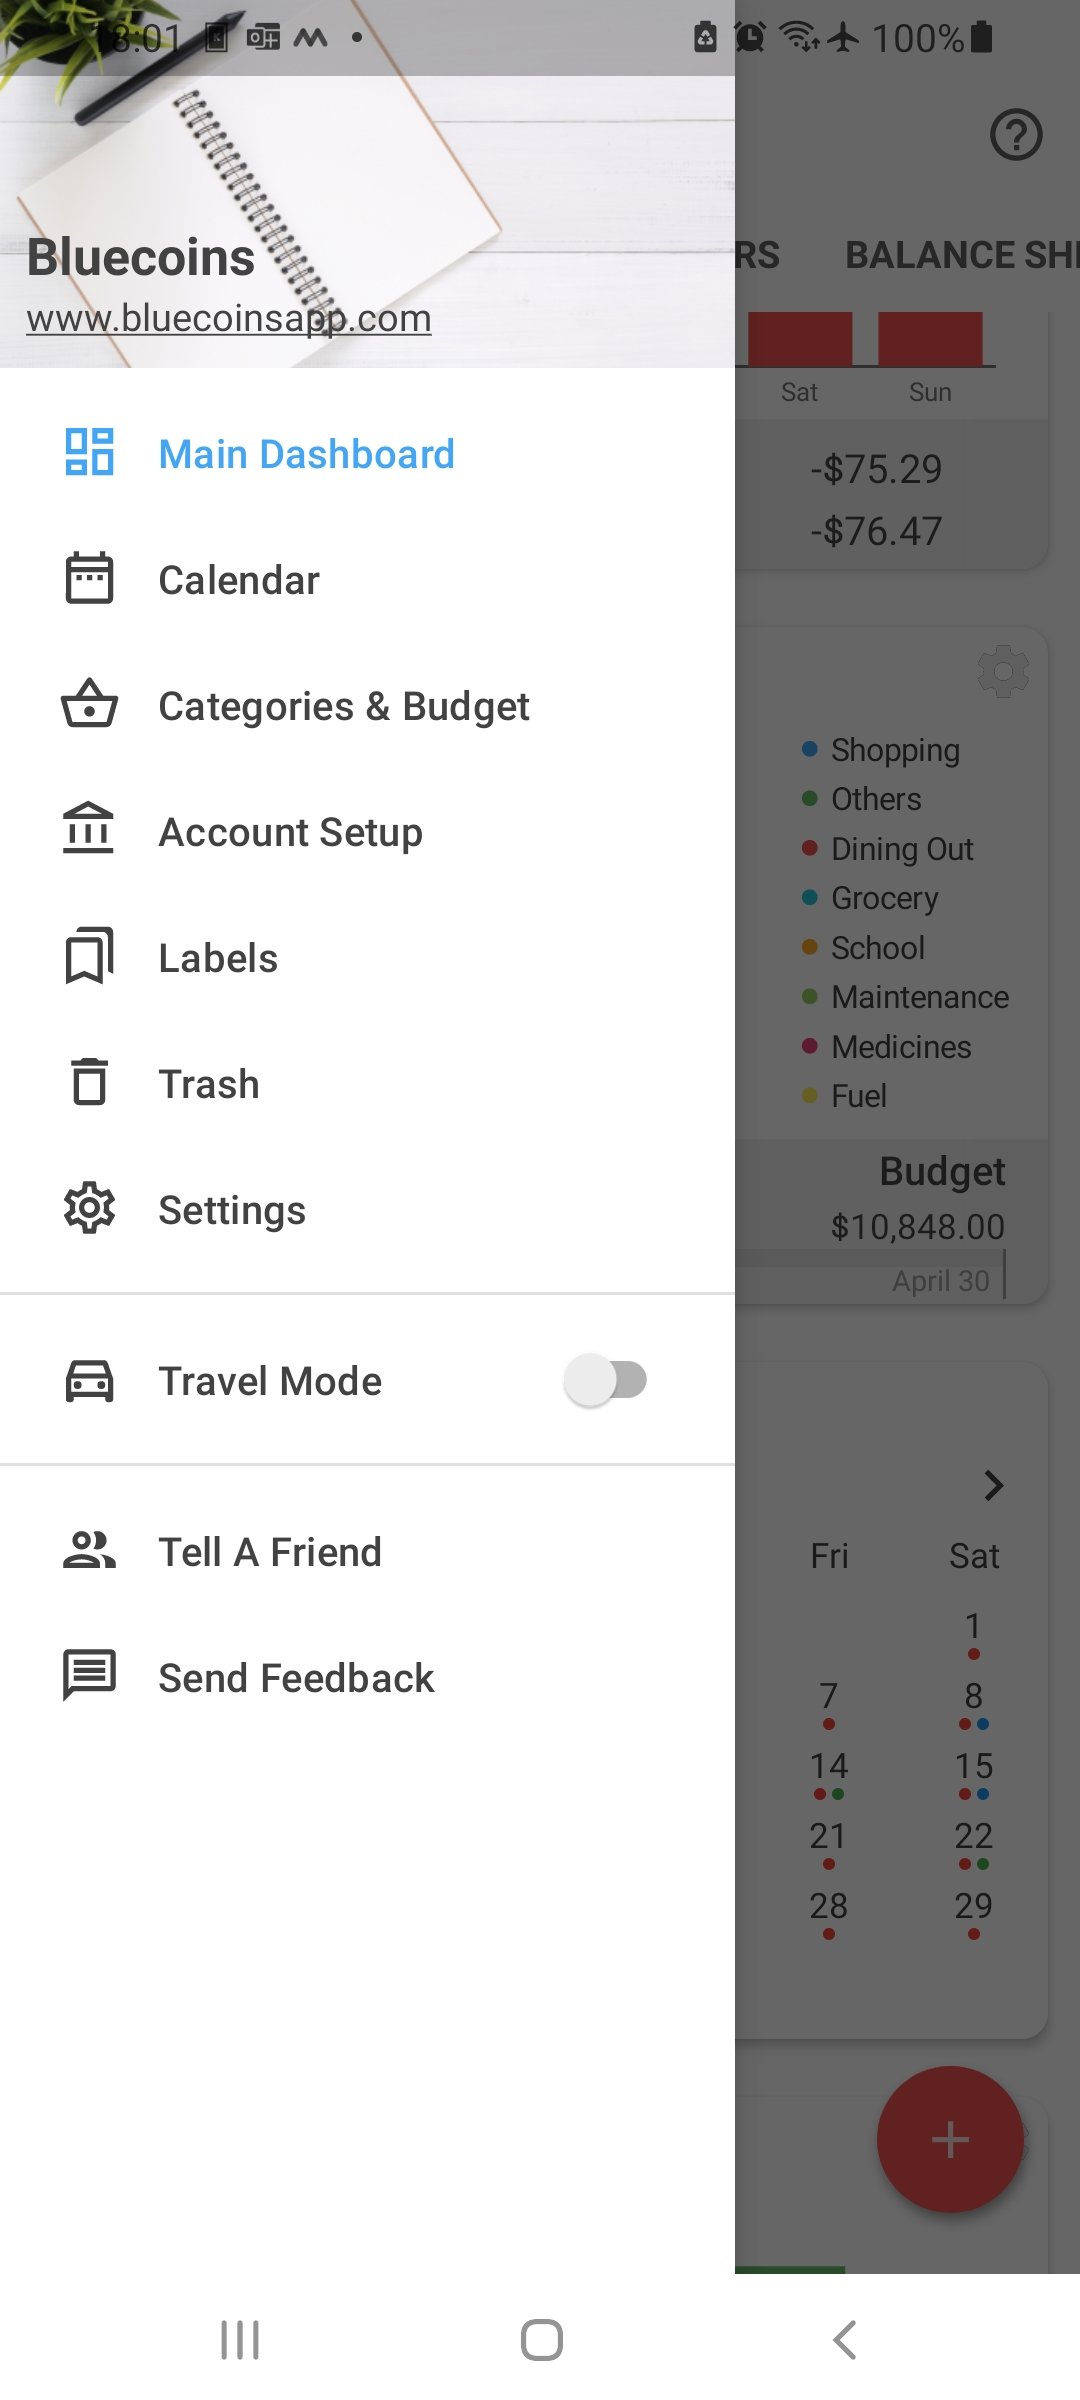
\includegraphics[width=\textwidth]{Screen Shots/BlueCoins/W_ItemMenu.jpg}
    \caption{Blue coins  main menu .}
    \label{fig:image2}
  \end{minipage}
\end{figure}

\newpage
\subsection{Money Lover}
\hspace{\parindent}Money Lover is a mobile application that allows users to manage their personal finances by tracking their expenses, creating budgets, and setting financial goals. The app offers features such as expense tracking, bill reminders, and budget planning. It also provides reports and insights to help users better understand their spending habits and financial situation.

\hspace{\parindent}Compared to BlueCoins, Money Lover places a greater emphasis on user experience, with a user-friendly interface that is easy to navigate and customize. It also offers a variety of customization options, such as the ability to choose between different themes and fonts. Additionally, Money Lover has a social feature that allows users to share expenses with friends and family, making it a useful tool for group expenses.

\hspace{\parindent}Although Money Lover is a robust application for personal finance management, it does have a heavier focus on its paid feature set. This could potentially make it less appealing to the average user who may not yet be ready to invest in additional features. 

\hspace{\parindent}Moreover, the app may be seen as contradictory to its purpose, as the expensive paid feature set may discourage users who are looking for a cost-effective and accessible solution. In comparison to other solutions, Money Lover may not be as user-friendly and intuitive, especially for those who prioritize simplicity and ease of use in their financial management applications.

\hspace{\parindent}While it is a comprehensive tool for managing personal finances, it leans more towards a paid feature set which may be less accessible for the average user. This may be a disadvantage for those who are just starting to manage their finances and are not yet willing or able to pay for additional features.

\begin{figure}[htbp]
  \centering
  \begin{minipage}[b]{0.27\textwidth}
    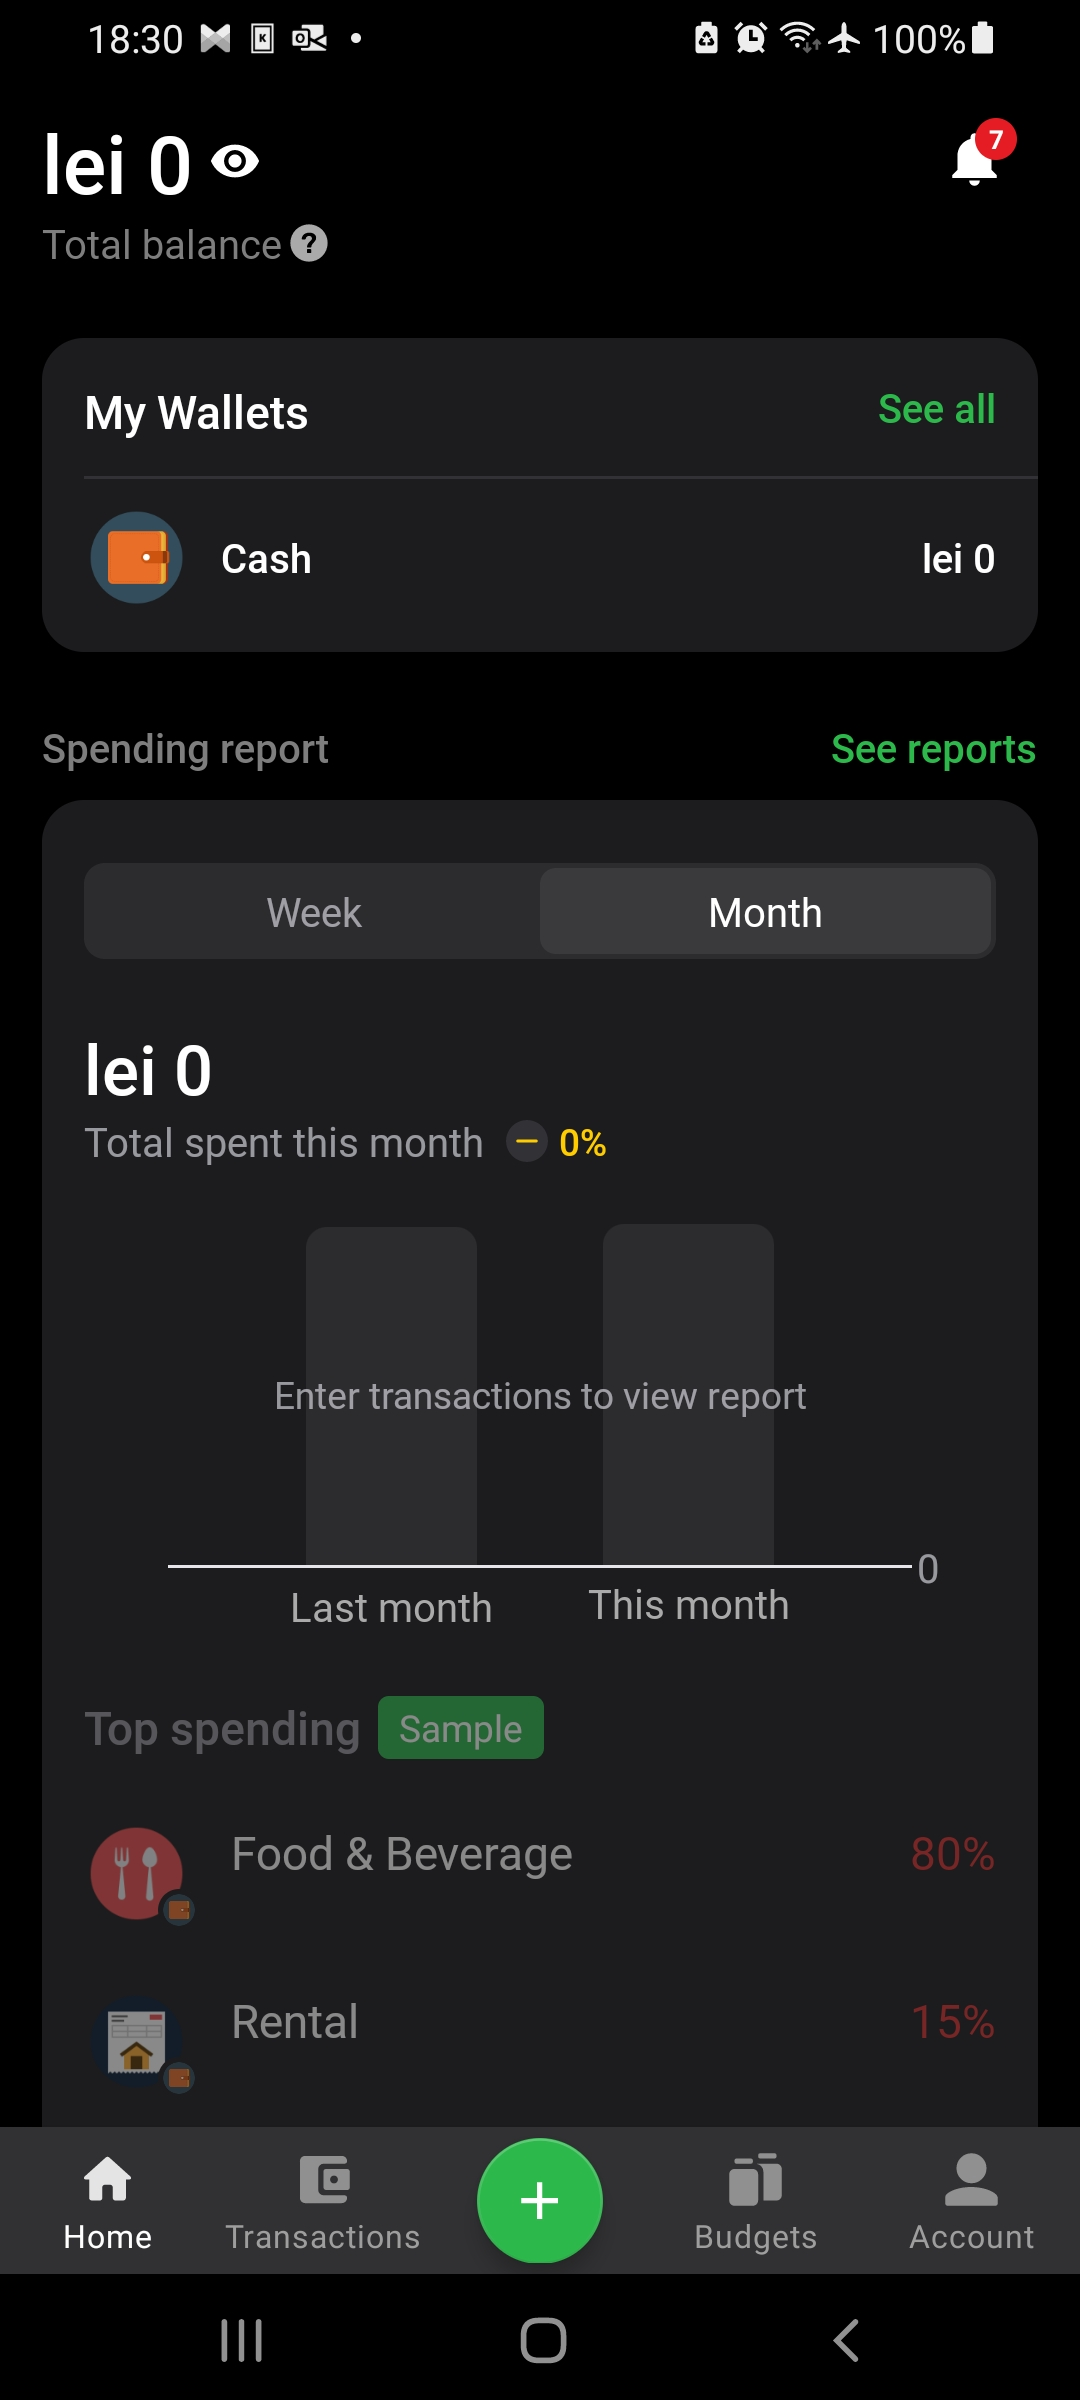
\includegraphics[width=\textwidth]{Screen Shots/MoneyLover/D_MainMenu.jpg}
    \caption{Money Lover main menu 1.}
    \label{fig:image1}
  \end{minipage}
  \hfill
  \begin{minipage}[b]{0.27\textwidth}
    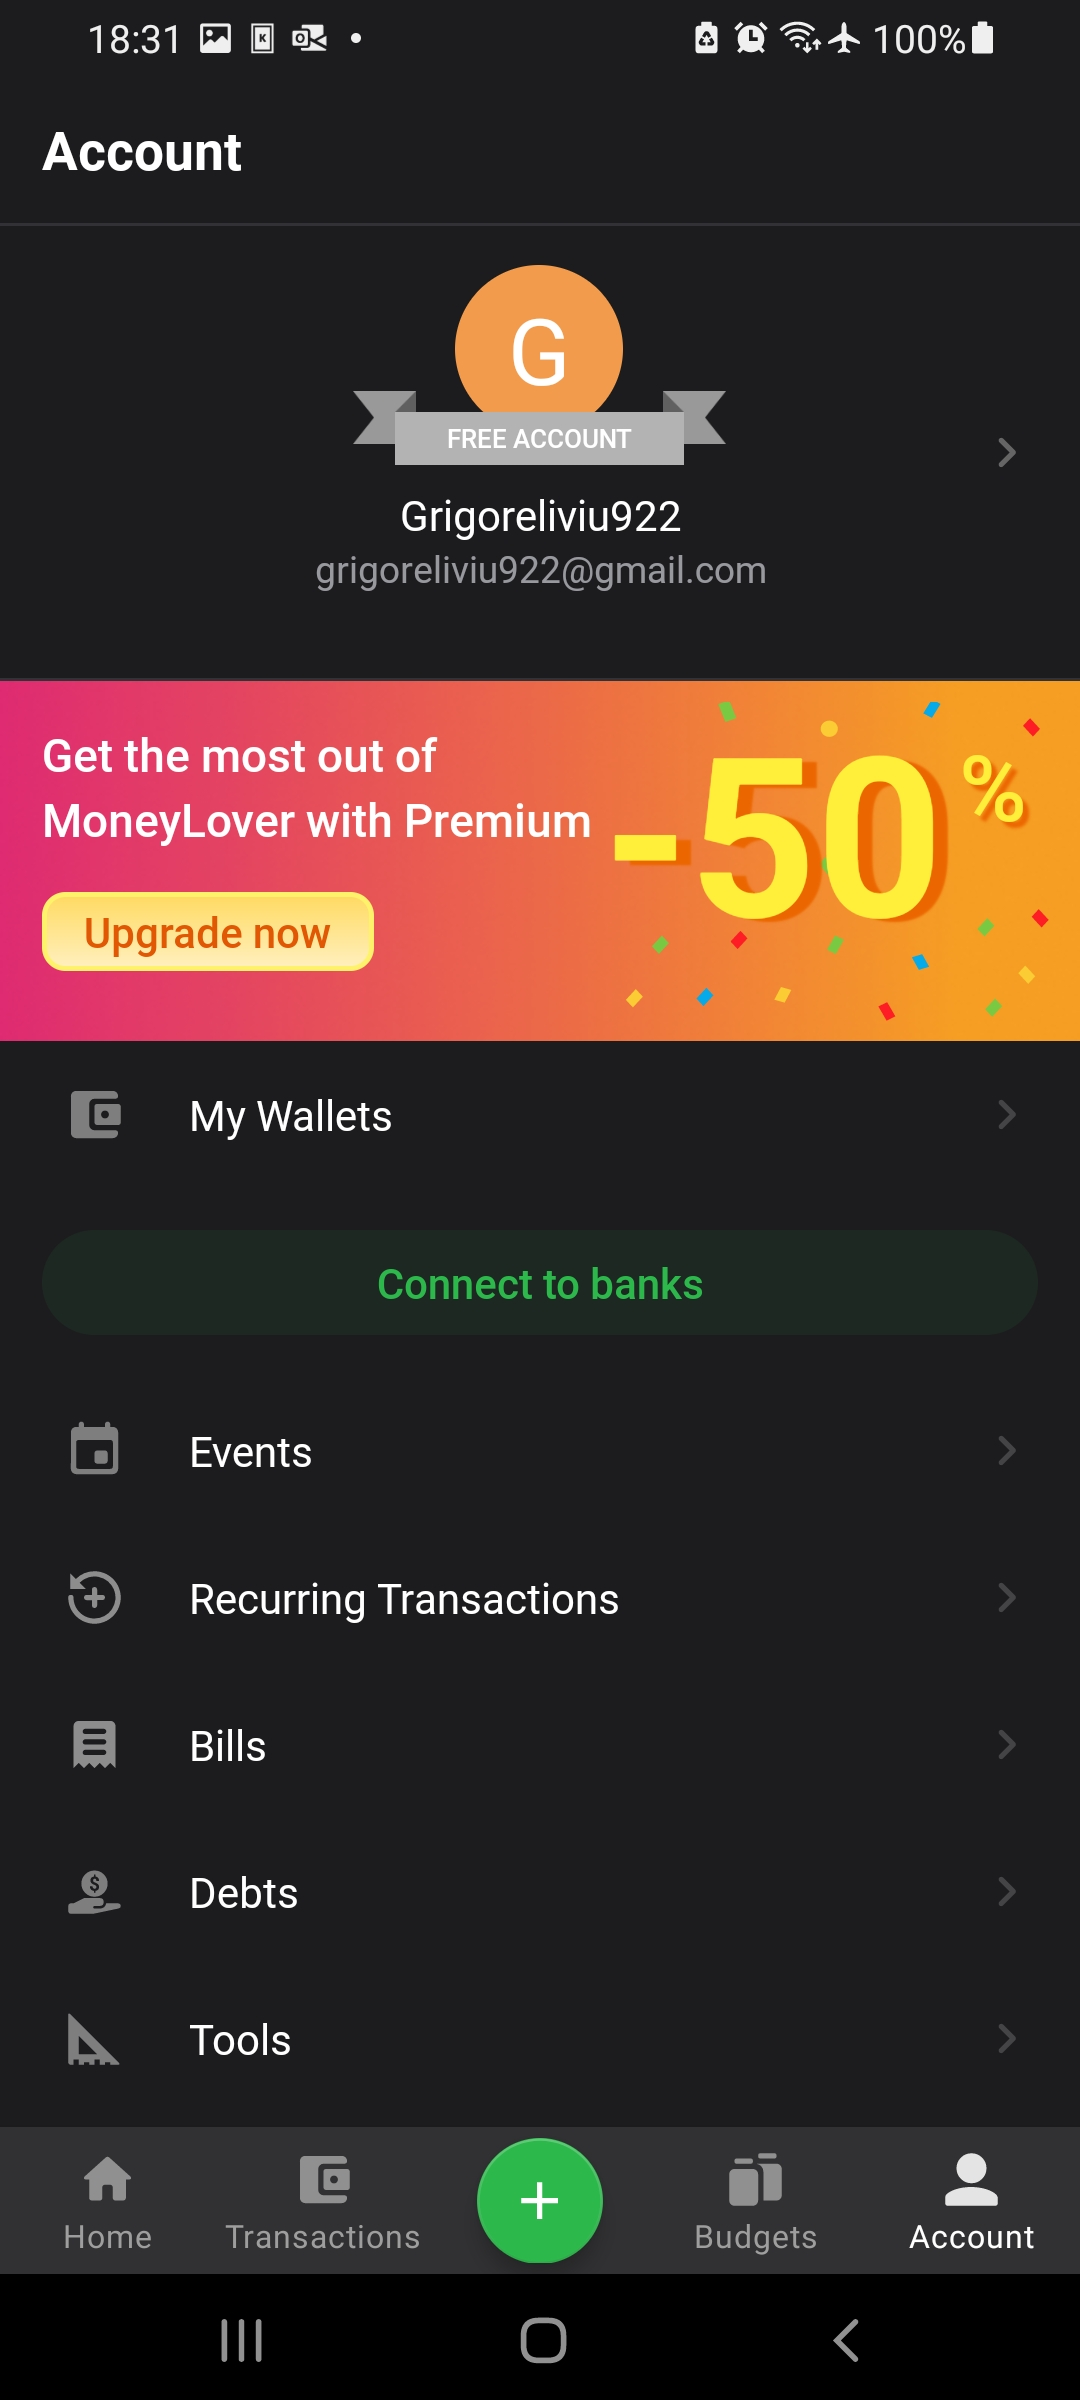
\includegraphics[width=\textwidth]{Screen Shots/MoneyLover/Account.jpg}
    \caption{Money Lover account screen.}
    \label{fig:image2}
  \end{minipage}
\end{figure}
\newpage




\subsection{Revolut}
\hspace{\parindent}Revolut is a financial technology company that provides a mobile application for managing finances, including money transfers, currency exchange, and investment services. The app allows users to hold and exchange money in different currencies at the interbank exchange rate, making it a popular choice for international transactions.

\hspace{\parindent}While Revolut may not be a direct competitor to the proposed money management application, it is worth mentioning as it is a popular choice among users for managing their finances. The app's user-friendly interface and innovative features have made it a popular choice among millennials and tech-savvy users.

\hspace{\parindent}One advantage of Revolut is its focus on security and fraud prevention. The app offers features such as disposable virtual cards and transaction notifications to help users detect and prevent fraudulent activities. However, one disadvantage of Revolut is its limited support for certain countries and currencies, which may be a drawback for users who require more flexibility in their financial management options.

\hspace{\parindent}Overall, while Revolut may not be a direct competitor to the proposed money management application, its success and popularity among users highlight the importance of user-friendly interfaces and innovative features in the financial technology industry.

\begin{figure}[htbp]
  \centering
  \begin{minipage}[b]{0.27\textwidth}
    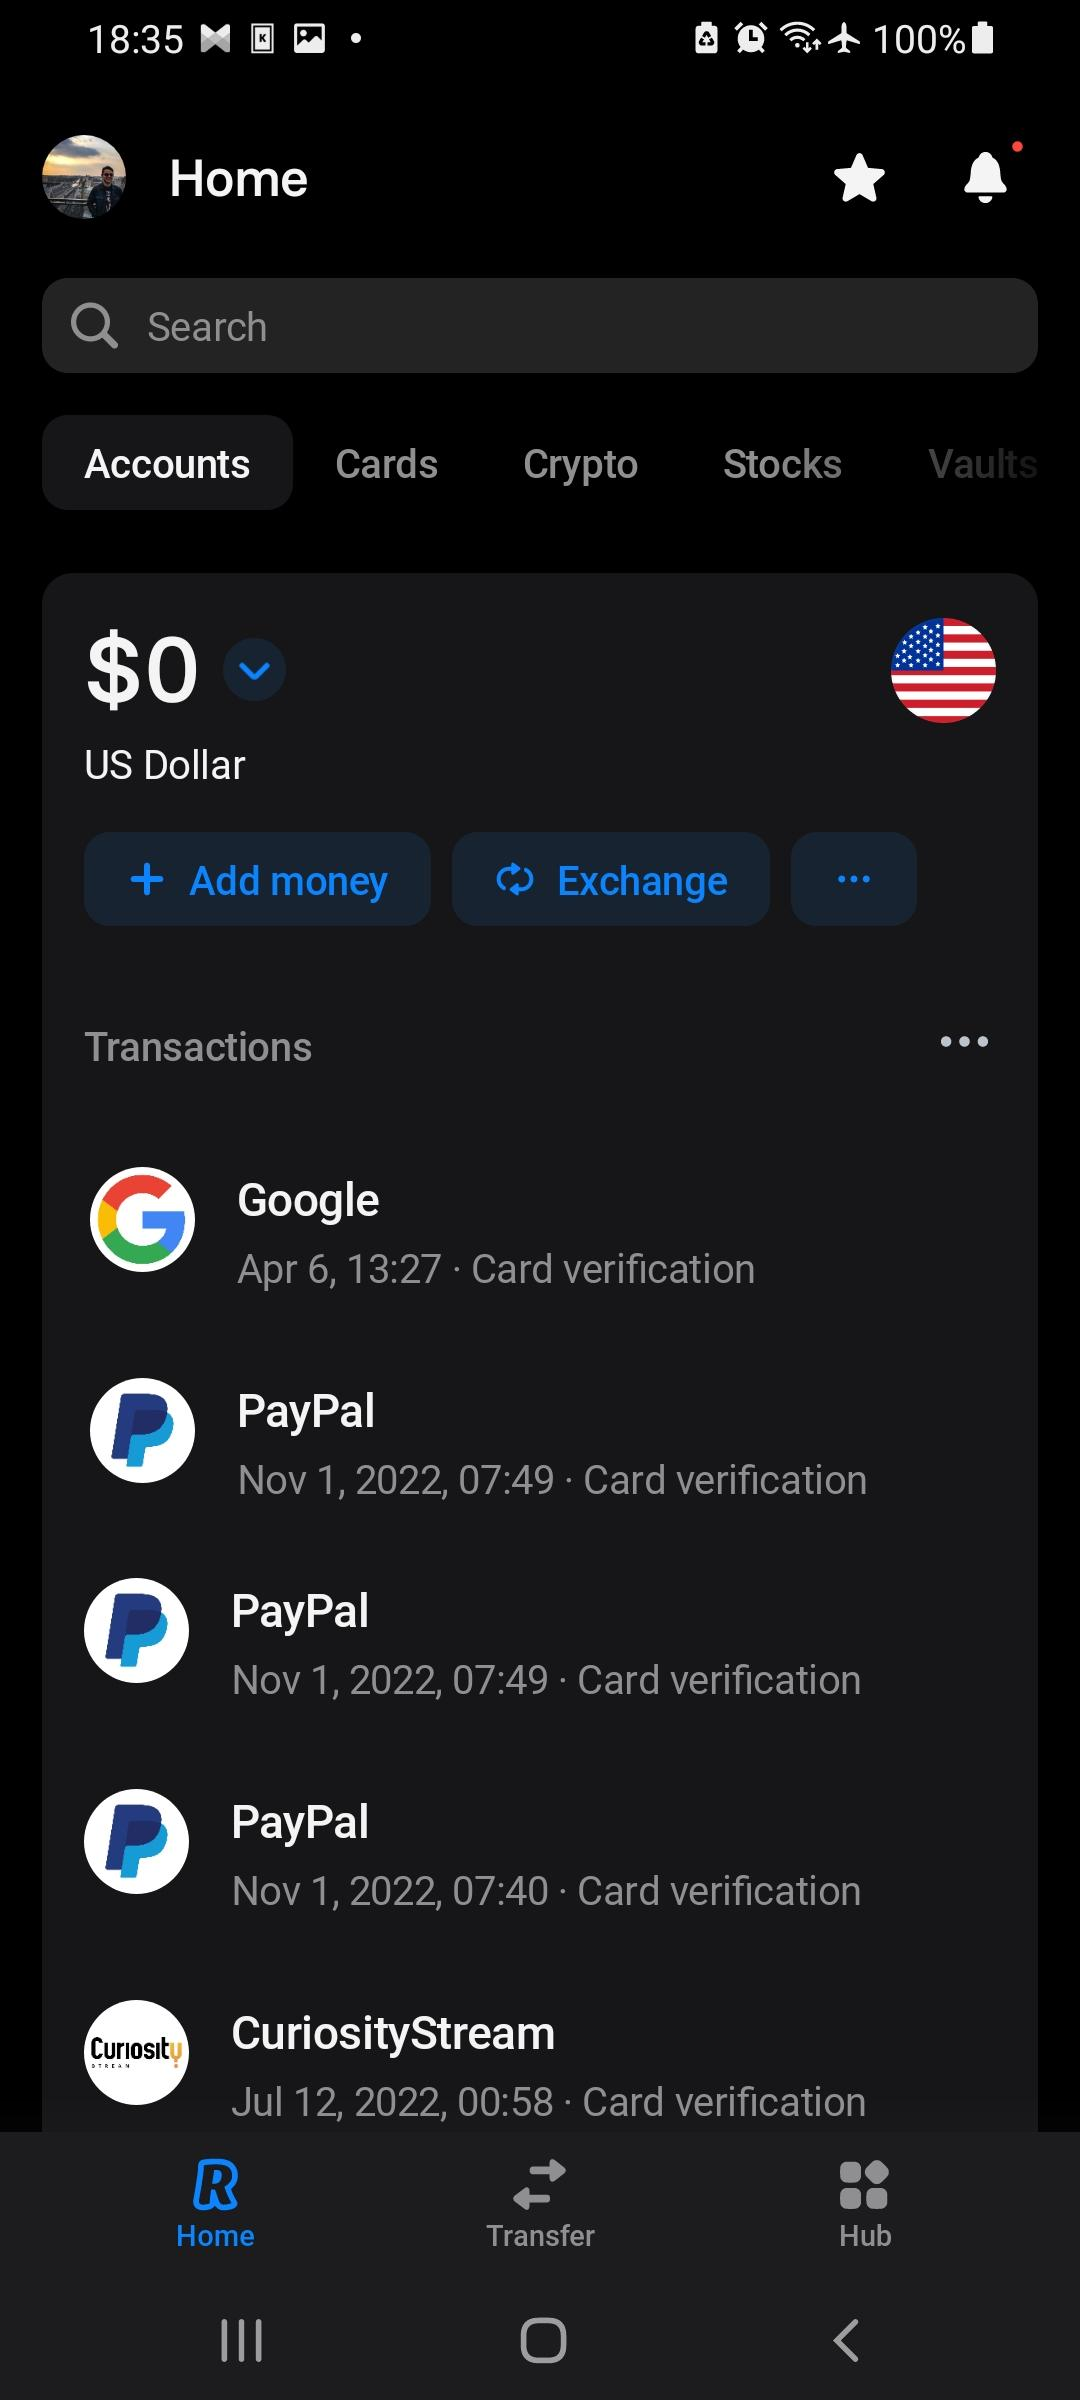
\includegraphics[width=\textwidth]{Screen Shots/Revolut/D_Revolut.jpg}
    \caption{Revolut Dark main menu 1.}
    \label{fig:image1}
  \end{minipage}
  \hfill
  \begin{minipage}[b]{0.27\textwidth}
    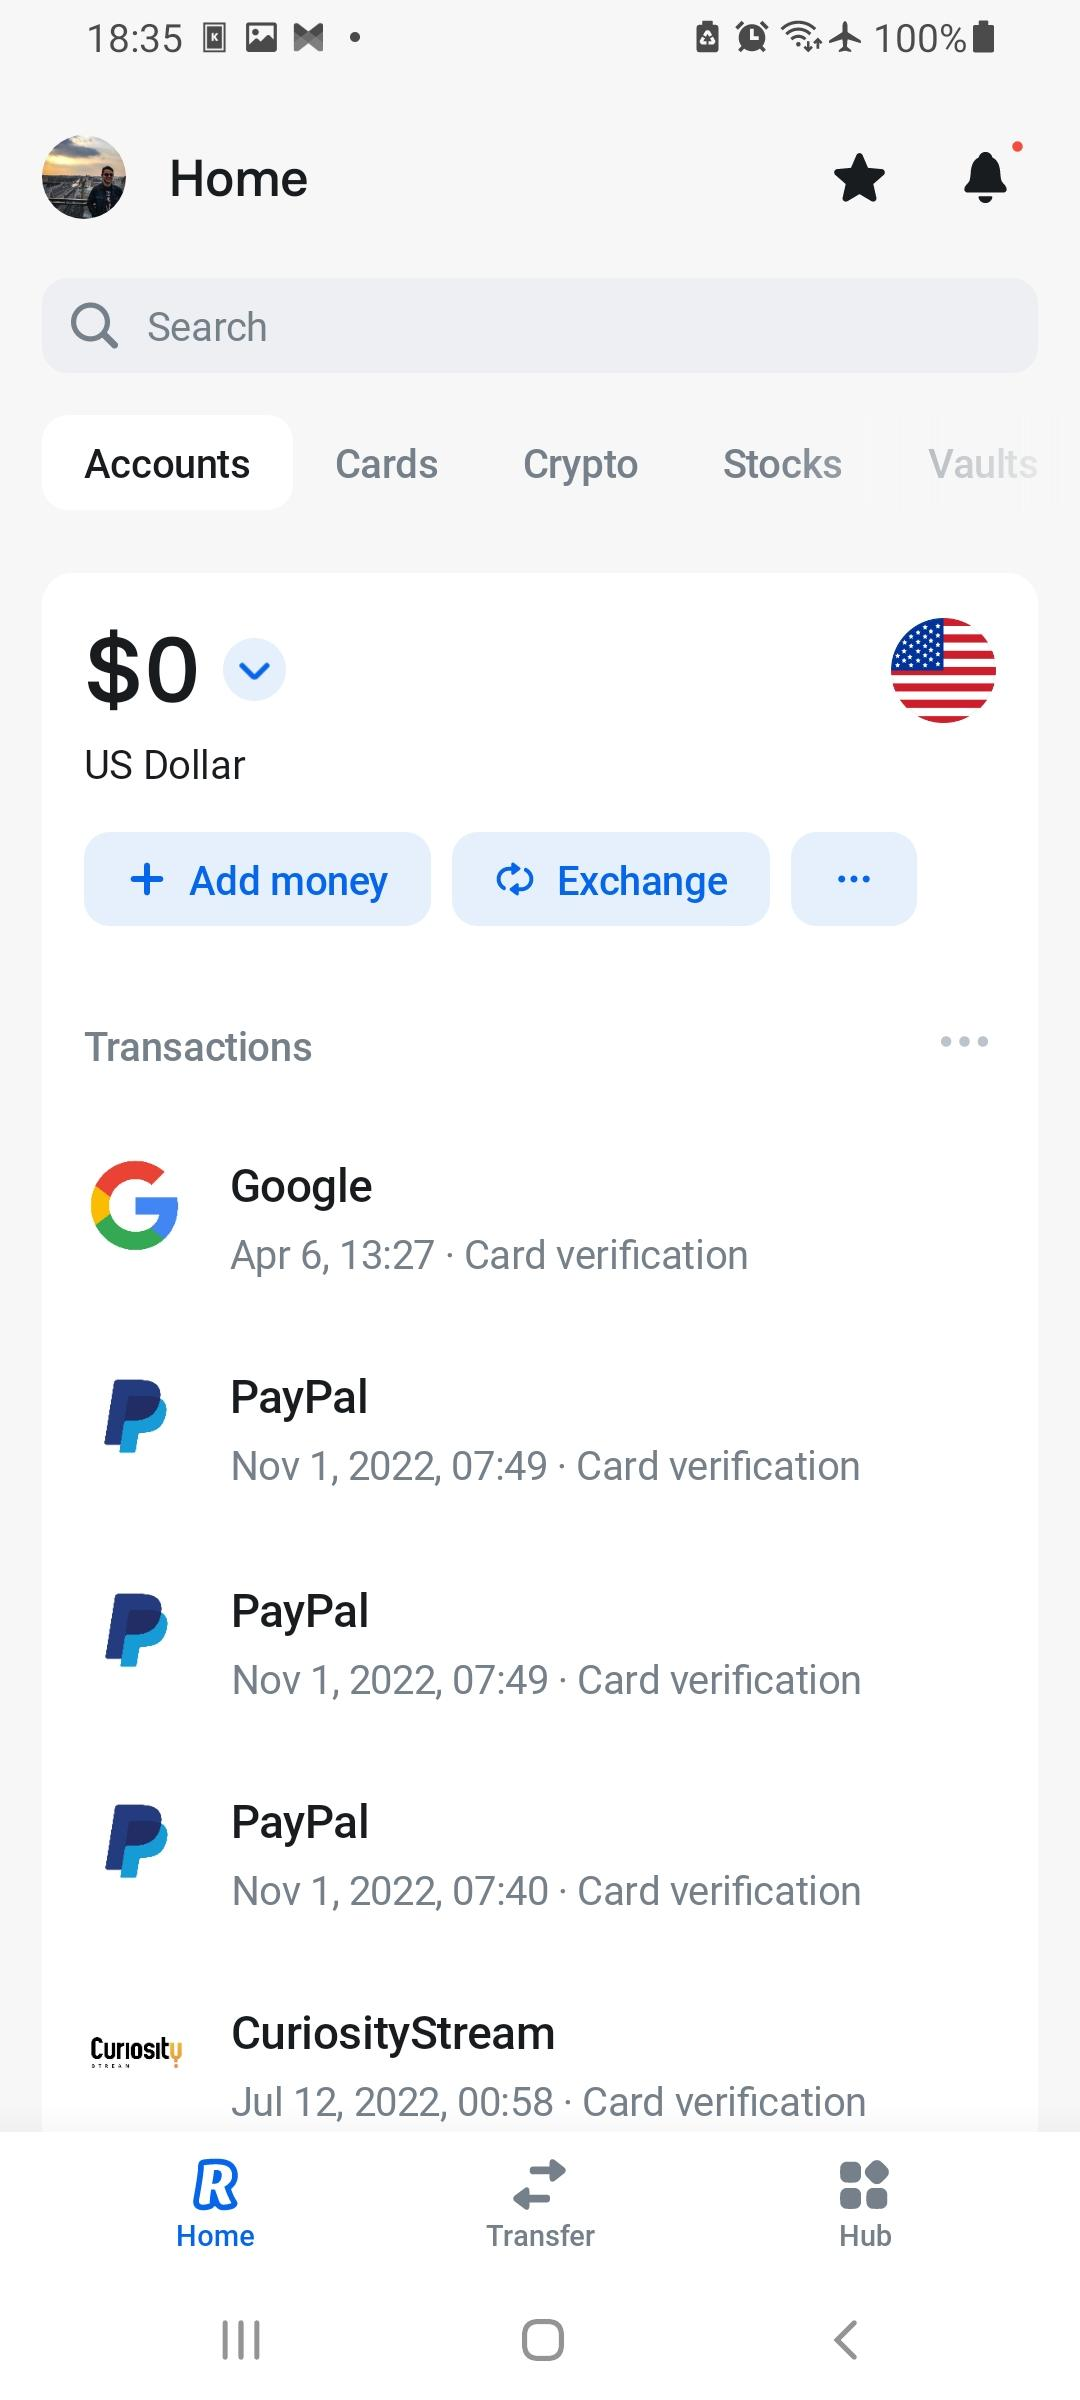
\includegraphics[width=\textwidth]{Screen Shots/Revolut/W_Revolut.jpg}
    \caption{Revolut main menu .}
    \label{fig:image2}
  \end{minipage}
\end{figure}
